\chapter{Simplified Parametrisation of the Spiral}
\label{sec:parametrisierung}
\section{Motivation for the New Parametrisation}
The constants \(\frac{6}{\pi\sqrt{3}}\) and \(\frac{\pi}{\sqrt{3}}\) arise
directly from the asymptotic structure of the arc length of the Archimedean spiral
\(r(\theta)=a\theta\). The exact arc-length function reads


\[
L(\theta)=\frac{a}{2}\bigl[\theta\sqrt{\theta^{2}+1}+\operatorname{arcsinh}(\theta)\bigr].
\]


For large \(\theta\) the term \(\theta\sqrt{\theta^{2}+1}\) dominates, so that


\[
L(\theta)\sim \frac{a}{2}\theta^{2}.
\]


With \(a=\frac{6}{\pi^{2}}\) the asymptotic relation


\[
L(\theta)\sim \frac{3}{\pi^{2}}\theta^{2}
\]


follows.

Introducing a parameter \(p\) that represents the arc length, the inversion
of \(p=L(\theta)\) yields


\[
\theta(p)\approx \sqrt{\frac{2p}{a}}
= \frac{\pi}{\sqrt{3}}\sqrt{p}.
\]


The constant \(\sqrt{3}\) thus arises directly from the quadratic
growth rate of the arc length and represents the scaling factor that
ensures the asymptotic identification of the parameter with the arc length.

Since \(r=a\theta\), the radius becomes


\[
r(p)=a\,\theta(p)
= \frac{6}{\pi^{2}}\cdot\frac{\pi}{\sqrt{3}}\sqrt{p}
= \frac{6}{\pi\sqrt{3}}\sqrt{p}.
\]



The constant \(\sqrt{3}\) thus possesses an intrinsic geometric meaning:
it characterises the scaling required to reparametrise the
spiral so that the new parameter \(p\) produces equidistant arc lengths.
The same value appears in the analysis of the quadratic function $f(x) = \tfrac{1}{6}(2x^2+3x+1)$ as the horizontal stretching factor $\sqrt{3}$ associated with its leading coefficient $\tfrac13$; both occurrences of $\sqrt{3}$ thus trace back to the same fraction $2/6$ in the definition of $k(n)$.


\begin{tcolorbox}[
  title={Why a new parametrisation is necessary},
  colback=gray!5,
  colframe=gray!50!black,
  enhanced,
  breakable
]
The standard parametrisation of the Archimedean spiral via the angle \(\theta\)
describes the curve geometrically correctly but does not produce arc lengths
that correspond to the arithmetic structure of the sequence \(k(n)\). For the
present application a parameter is needed whose increment corresponds directly
to the arc length measured along the spiral. By introducing the parameter \(p\),
which runs through the values of \(k(n)\), an equidistant arc-length scale arises. Precisely: $p$ is exactly the value parameter of the sequence and asymptotically its arc length; the deviation is quantified in Chapter~\ref{sec:bogenlaenge_spirale}.
The spiral remains geometrically unchanged but acquires a parametrisation that
precisely reflects the arithmetic structure of the sequence.
\end{tcolorbox}


\begin{figure}[htbp]
  \centering
  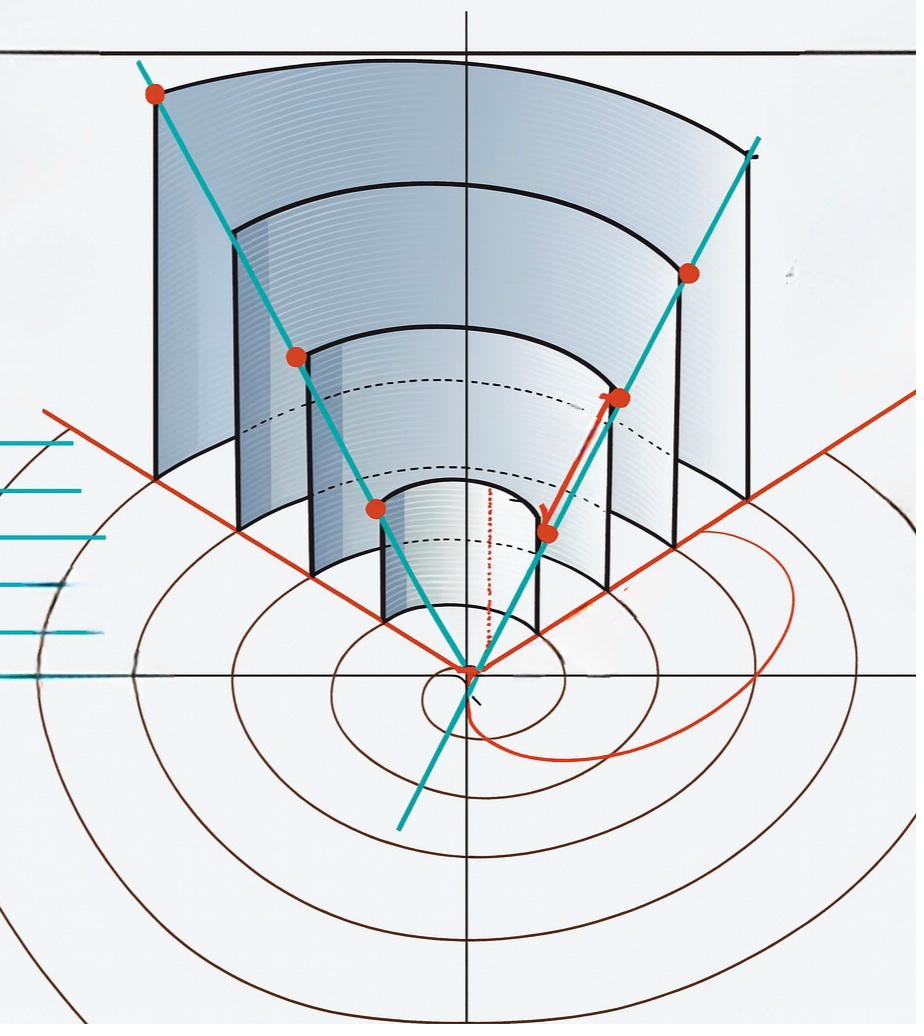
\includegraphics[width=0.78\textwidth]{bilder/spirale_3d_uebergang}
  \caption{Transition from the two-dimensional Archimedean spiral (bottom)
    to the three-dimensional cylindrical structure (top). The cyan rays
    mark the radius vector $r(\theta)$ at the integer points of the
    sequence; the orange lines visualise the corresponding tangential directions.
    The concentrically arranged circular arcs correspond to the discrete
    radial increments $\Delta r = 12/\pi$, which, upon unrolling, become the
    vertical spacings of the 3D surface.}
  \label{fig:spirale_3d_uebergang}
\end{figure}

\section{Polar Form with Parameter \texorpdfstring{$p$}{p}}

We introduce a new parameter $p$ that directly corresponds to the integer
function values of the sequence $k(n)$.

\begin{theorem}[Simplified polar representation]
The spiral can be expressed in the form
\begin{equation}
\boxed{
\begin{aligned}
r(p) &= \frac{6}{\pi} \cdot \sqrt{\frac{p}{3}} \\
     &= \frac{6}{\pi\sqrt{3}} \cdot \sqrt{p}, \\[6pt]
\theta(p) &= \pi \cdot \sqrt{\frac{p}{3}} \\
          &= \frac{\pi}{\sqrt{3}} \cdot \sqrt{p}
\end{aligned}
}
\end{equation}
where $p$ runs through the values of the sequence $k(n)$.
\end{theorem}

With numerical values:
\begin{align}
r(p) &= \frac{6}{\pi\sqrt{3}} \cdot \sqrt{p} \approx 1.102657790844 \cdot \sqrt{p}, \\
\theta(p) &= \frac{\pi}{\sqrt{3}} \cdot \sqrt{p} \approx 1.813799364234 \cdot \sqrt{p}.
\end{align}

\begin{note}
A common source of error is the confusion of the two equivalent forms
of the radius function. One has
\[
  r(p) = \frac{6}{\pi\sqrt{3}}\,\sqrt{p}
       = \frac{6}{\pi}\,\sqrt{\frac{p}{3}}.
\]
The factor $\frac{6}{\pi} \approx 1.9099$ is the coefficient of $\sqrt{p/3}$, \emph{not} 
of $\sqrt{p}$. If it is multiplied directly by $\sqrt{p}$, the resulting 
coordinates are too large by a factor of $\sqrt{3} \approx 1.732$. 
For numerical evaluation it is therefore advisable to use the form 
$r(p) = 1.102657790844 \cdot \sqrt{p}$.
\end{note}

\section[Parametric Representation in Cartesian Coordinates]{Parametric Representation\texorpdfstring{\\}{ }in Cartesian Coordinates}

\begin{equation}
\begin{aligned}
x(p) &= r(p)\cos(\theta(p))
     = \frac{6}{\pi\sqrt{3}}\sqrt{p}\,
       \cos\!\left(\frac{\pi}{\sqrt{3}}\sqrt{p}\right), \\[6pt]
y(p) &= r(p)\sin(\theta(p))
     = \frac{6}{\pi\sqrt{3}}\sqrt{p}\,
       \sin\!\left(\frac{\pi}{\sqrt{3}}\sqrt{p}\right).
\end{aligned}
\end{equation}

\begin{remark}[The angular factor as a Dirichlet $L$-value:
Eisenstein integers]
\label{rem:eisenstein_L}
The angular factor $\pi/\sqrt{3}$ of the $p$-parametrisation admits an
exact expression through a Dirichlet $L$-function. Let $\chi_{-3}$ be
the nontrivial character modulo~$3$, i.e.\ $\chi_{-3}(n) = +1$ for
$n \equiv 1 \pmod 3$, $-1$ for $n \equiv 2 \pmod 3$, and $0$ for
$3 \mid n$. Its $L$-series at $s=1$,
\begin{equation}\label{eq:L_chi3}
  L(1,\chi_{-3})
  = 1 - \frac12 + \frac14 - \frac15 + \frac17 - \frac18 + \cdots
  = \frac{\pi}{3\sqrt{3}},
\end{equation}
is a classical evaluation; by Dirichlet's class number formula it reads
\[
  L(1,\chi_{-3}) = \frac{2\pi h}{w\sqrt{|d|}}
\]
with class number $h = 1$, discriminant $d = -3$ and $w = 6$ units for
the field $\mathbb{Q}(\sqrt{-3})$~\cite{IrelandRosen1990}. Hence
\begin{equation}\label{eq:angular_L}
  \frac{\pi}{\sqrt{3}} = 3\,L(1,\chi_{-3}) = \frac{w}{2}\,L(1,\chi_{-3}),
  \qquad
  \theta(p) = \frac{w}{2}\,L(1,\chi_{-3})\,\sqrt{p}.
\end{equation}

The ring of integers of $\mathbb{Q}(\sqrt{-3})$ is the ring of
Eisenstein integers $\mathbb{Z}[\omega]$, $\omega = e^{2\pi i/3}$ ---
the hexagonal lattice, whose unit group has order exactly~$6$. Its
arithmetic is organised by the same congruence classes as the present
work: a rational prime $p > 3$ splits in $\mathbb{Z}[\omega]$ if
$p \equiv 1 \pmod 3$ and remains inert if $p \equiv 2 \pmod 3$, while
$p = 3$ ramifies. For odd $n$, the classes $n \equiv 1, 5 \pmod 6$ on
which $k(n)$ is integer-valued are precisely the classes
$n \equiv 1, 2 \pmod 3$, so the two strands of the twin structure
correspond to the two splitting types. The associated Dedekind zeta
function factorises as
$\zeta_{\mathbb{Q}(\sqrt{-3})}(s) = \zeta(s)\,L(s,\chi_{-3})$.

It should be stated clearly what is established and what is not: the
identities \eqref{eq:L_chi3}--\eqref{eq:angular_L} are exact, and the
correspondence between the residue classes and the splitting law in
$\mathbb{Z}[\omega]$ is classical algebraic number theory. That the
angular factor of the spiral is forced to be this particular $L$-value
--- rather than merely equal to it through the shared origin of both
quantities in the modulus~$6$ --- is a conjecture of the present work
and remains open.
\end{remark}

\begin{remark}[The angular factor and the reflection formula of the
Gamma function]
\label{rem:gamma_reflection}
Euler's reflection formula
$\Gamma(z)\Gamma(1-z) = \pi/\sin(\pi z)$ yields at $z = \tfrac13$
\begin{equation}\label{eq:gamma_reflection}
  \Gamma\!\left(\tfrac13\right)\Gamma\!\left(\tfrac23\right)
  = \frac{\pi}{\sin(\pi/3)}
  = \frac{2\pi}{\sqrt{3}},
  \qquad\text{hence}\qquad
  \frac{\pi}{\sqrt{3}}
  = \frac{1}{2}\,\Gamma\!\left(\tfrac13\right)\Gamma\!\left(\tfrac23\right).
\end{equation}
The arguments $\tfrac13$ and $\tfrac23$ are the two residue classes
modulo~$3$ --- normalised to the unit interval --- that carry the twin
structure of $k(n)$; the angular factor is one half of the product of
the Gamma values at exactly these two points.

The appearance of $\sqrt{3}$ in \eqref{eq:gamma_reflection} and in the
$L$-value of Remark~\ref{rem:eisenstein_L} is not independent: the
Chowla--Selberg formula~\cite{ChowlaSelberg1967} expresses the periods
attached to the imaginary quadratic field $\mathbb{Q}(\sqrt{-3})$ in
terms of $\Gamma(\tfrac13)$, so that the $L$-value and the
Gamma product are two evaluations rooted in the same field. Within the
present work these identities are recorded as structure shared with
the parametrisation constants; no derivation of the spiral from either
side is claimed.
\end{remark}

\begin{remark}[The two roles of $L(s,\chi_{-3})$: value and spectrum]
\label{rem:L_two_roles}
The function $L(s,\chi_{-3})$ of Remark~\ref{rem:eisenstein_L} enters
the arithmetic of the classes $6k \pm 1$ a second time, through its
zeros. The nontrivial character modulo~$6$ is induced by the primitive
character $\chi_{-3}$ modulo~$3$, so that
\begin{equation}
  L(s,\chi_6) = L(s,\chi_{-3})\,\bigl(1 + 2^{-s}\bigr),
\end{equation}
and since the elementary factor $1 + 2^{-s}$ has no zeros in the
critical strip, both functions possess the same nontrivial zeros
(numerically, the lowest ones lie at $\gamma = 8.0397$, $11.2492$,
$15.7046$, $18.2620$, $20.4558$, \ldots).
By the explicit formulae of prime number theory~\cite{Davenport2000},
these zeros govern the fluctuation of the prime counts \emph{between}
the two residue classes: the combination
$\pi(x; 6, 1) - \pi(x; 6, 5)$ is a superposition of oscillations
$x^{\beta}\cos(\gamma \ln x)$ over the zeros $\beta + i\gamma$ of
$L(s,\chi_{-3})$, and the generalised Riemann hypothesis is the
statement that all these oscillations carry the minimal weight
$\beta = \tfrac12$.

The same $L$-function therefore acts on the present construction in
two distinct roles: its \emph{value} at $s = 1$ fixes the angular
factor of the parametrisation
(Remark~\ref{rem:eisenstein_L}), while its \emph{zeros} form the
frequency spectrum that modulates how the primes distribute themselves
between the two strands parametrised by it. The first role is a proven
identity; that the coincidence of the two roles carries structural
content is an open question of this work.
\end{remark}


\section{Derivatives}

\begin{theorem}[Derivatives of the polar coordinates]
\begin{equation}
\begin{aligned}
\frac{dr}{dp}
  &= \frac{d}{dp}\left[\frac{6}{\pi\sqrt{3}}\sqrt{p}\right]
   = \frac{6}{\pi\sqrt{3}} \cdot \frac{1}{2\sqrt{p}}
   = \frac{\sqrt{3}}{\pi\sqrt{p}}, \\[10pt]
\frac{d\theta}{dp}
  &= \frac{d}{dp}\left[\frac{\pi}{\sqrt{3}}\sqrt{p}\right]
   = \frac{\pi}{\sqrt{3}} \cdot \frac{1}{2\sqrt{p}}
   = \frac{\pi}{2\sqrt{3}\sqrt{p}}.
\end{aligned}
\end{equation}
\end{theorem}

Numerically:
\begin{align}
\frac{dr}{dp} &= \frac{\sqrt{3}}{\pi\sqrt{p}} = \frac{0.551328895422}{\sqrt{p}}, \\[4pt]
\frac{d\theta}{dp} &= \frac{\pi}{2\sqrt{3}\sqrt{p}} = \frac{0.906899682117}{\sqrt{p}}.
\end{align}
